\section{Auswertung}%
\label{sec:auswertung}
% {\lstinputlisting[firstline=1,lastline=1]{build/lin_verst_01__r1_200__rn_470__u1_100.txt}}
% {\lstinputlisting[firstline=2,lastline=2]{build/lin_verst_01__r1_200__rn_470__u1_100.txt}}
\subsection{Linearer Verst\"arker}

\begin{figure}[ht]
  \centering
  \input{build/lin_verst_01__r1_200__rn_470__u1_100.pgf}
  \caption{Linearer Verst\"arker mit $R_1 = \SI{200}{\kilo\ohm}$, $R_N = \SI{470}{\kilo\ohm}$.}
  \label{fig:}
\end{figure}

\begin{figure}[ht]
  \centering
  \input{build/lin_verst_02__r1_200__rn_100__u1_100.pgf}
  \caption{Linearer Verst\"arker mit $R_1 = \SI{200}{\kilo\ohm}$, $R_N = \SI{100}{\kilo\ohm}$}
  \label{fig:}
\end{figure}

\begin{figure}[ht]
  \centering
  \input{build/lin_verst_03__r1_100__rn_470__u1_100.pgf}
  \caption{Linearer Verst\"arker mit $R_1 = \SI{100}{\kilo\ohm}$, $R_N = \SI{470}{\kilo\ohm}$}
  \label{fig:}
\end{figure}

\begin{figure}[ht]
  \centering
  \input{build/lin_verst_04__r1_470__rn_100__u1_100.pgf}
  \caption{Linearer Verst\"arker mit $R_1 = \SI{470}{\kilo\ohm}$, $R_N = \SI{100}{\kilo\ohm}$}
  \label{fig:}
\end{figure}

\subsection{Integrator}
\begin{figure}[ht]
  \centering
  \input{build/integrator.pgf}
  \caption{}
  \label{fig:}
\end{figure}
\begin{figure}[ht]
  \centering
  \begin{subfigure}[]{\textwidth}
    \centering
    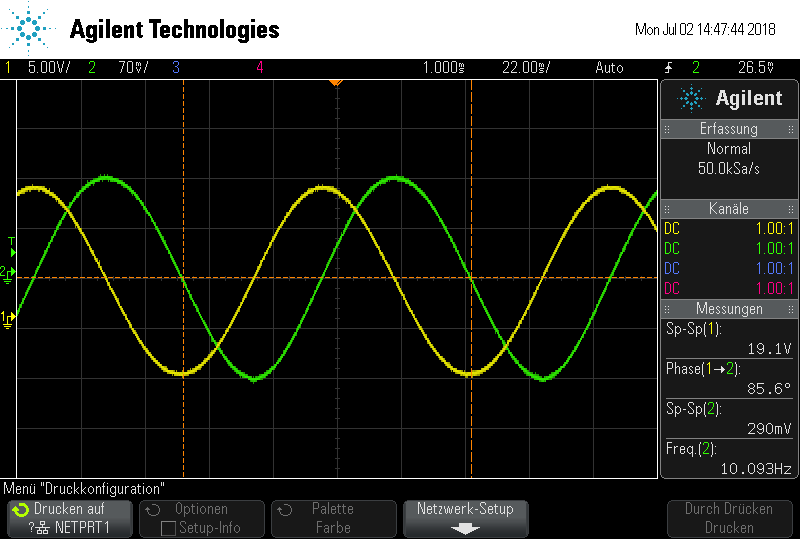
\includegraphics[height=0.3\textheight]{data/scope_262.png}
    \caption{Integration einer Sinusspannung.}
    \label{subfig:int_sinus}
  \end{subfigure}
  \begin{subfigure}[]{\textwidth}
    \centering
    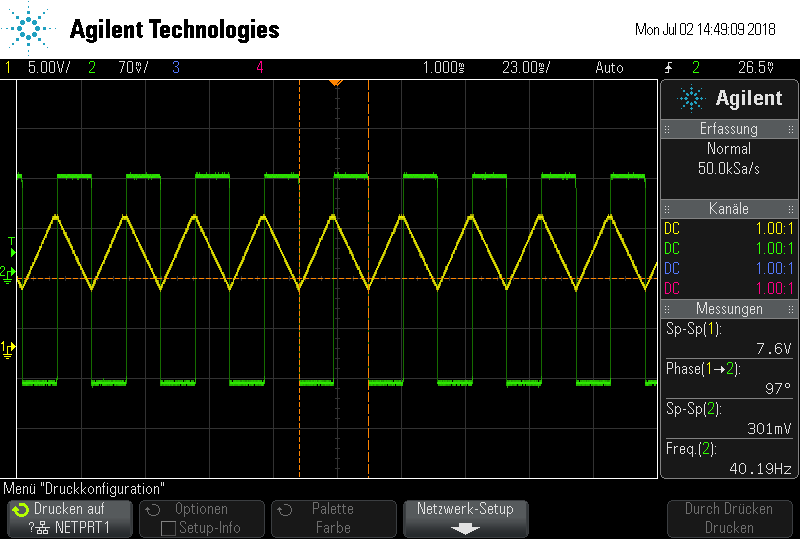
\includegraphics[height=0.3\textheight]{data/scope_263.png}
    \caption{Integration einer Rechteckspannung.}
    \label{subfig:int_rechteck}
  \end{subfigure}
  \begin{subfigure}[]{\textwidth}
    \centering
    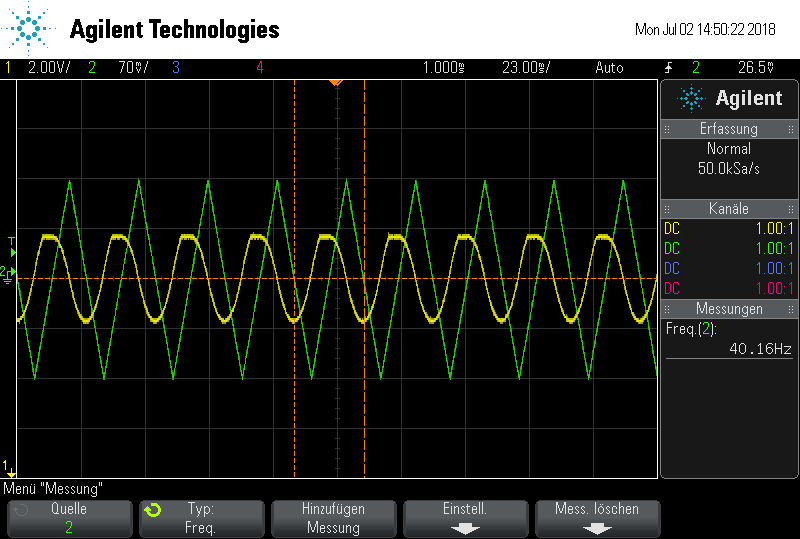
\includegraphics[height=0.3\textheight]{data/scope_264.png}
    \caption{Integration einer Dreiecksspannung.}
    \label{subfig:int_dreieck}
  \end{subfigure}
  \caption{Aufnahmen des Oszillopskops von verschiedenen Integrationen.}
  \label{fig:integrationen}
\end{figure}

\subsection{Differentiator}
\begin{figure}[ht]
  \centering
  \input{build/differentiator.pgf}
  \caption{}
  \label{fig:}
\end{figure}
\begin{figure}[ht]
  \centering
  \begin{subfigure}[]{\textwidth}
    \centering
    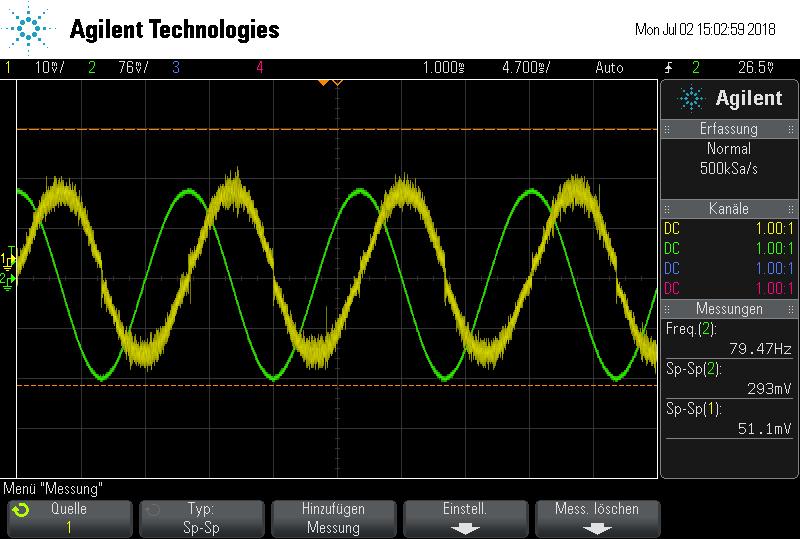
\includegraphics[height=0.3\textheight]{data/scope_265.png}
    \caption{Differentiation einer Sinusspannung.}
    \label{subfig:dif_sinus}
  \end{subfigure}
  \begin{subfigure}[]{\textwidth}
    \centering
    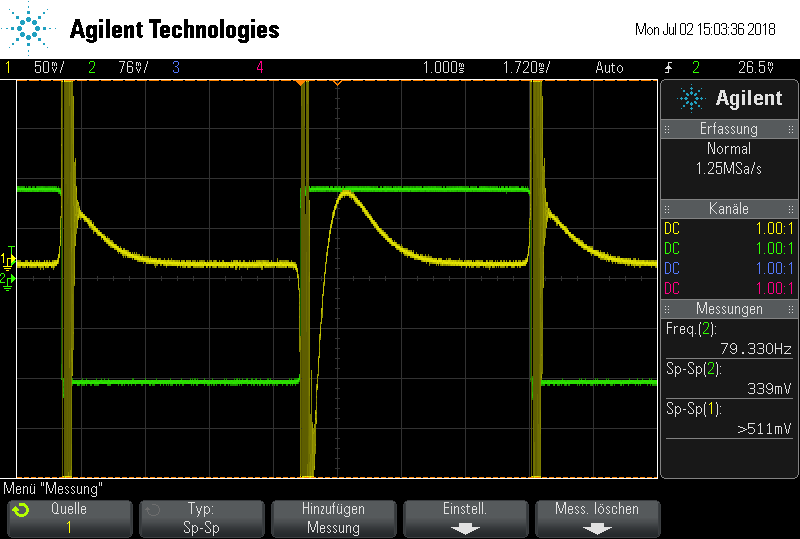
\includegraphics[height=0.3\textheight]{data/scope_266.png}
    \caption{Differentiation einer Rechteckspannung.}
    \label{subfig:dif_rechteck}
  \end{subfigure}
  \begin{subfigure}[]{\textwidth}
    \centering
    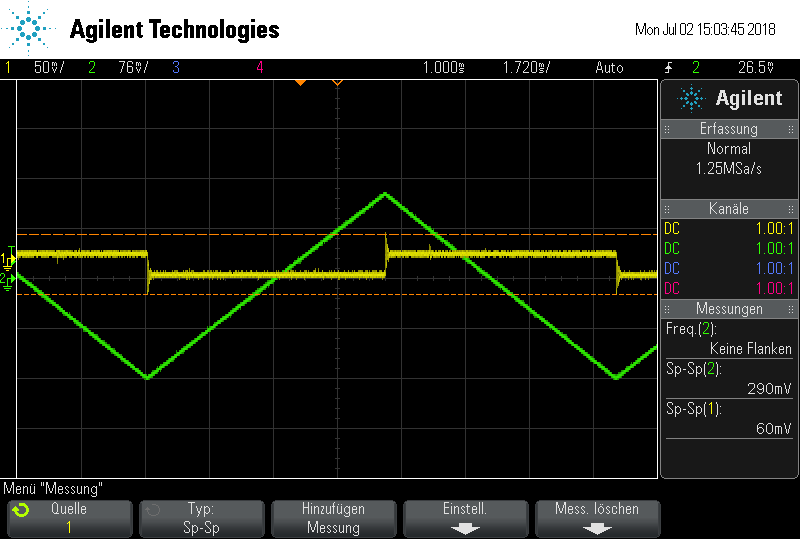
\includegraphics[height=0.3\textheight]{data/scope_267.png}
    \caption{Differentiation einer Dreiecksspannung.}
    \label{subfig:dif_dreieck}
  \end{subfigure}
  \caption{Aufnahmen des Oszillopskops von verschiedenen Differentiationen.}
  \label{fig:integrationen}
\end{figure}

\subsection{Schmitt-Trigger}
\begin{figure}[ht]
  \centering
  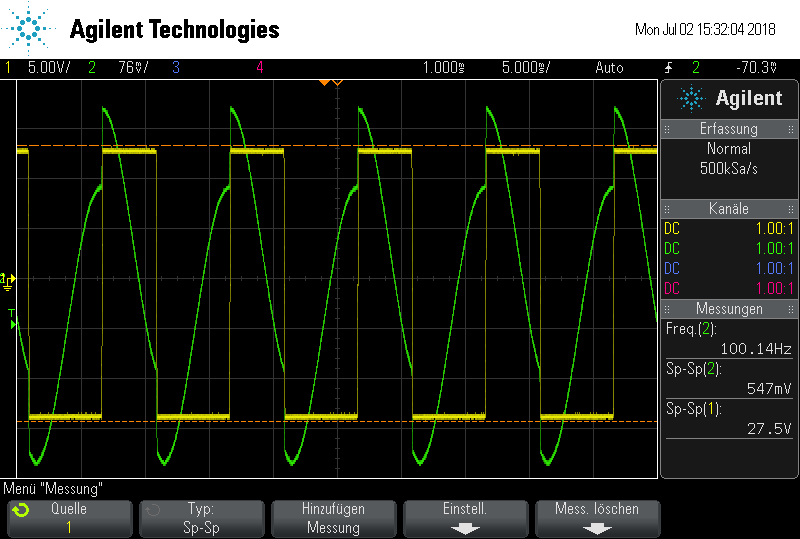
\includegraphics[height=0.3\textheight]{data/scope_268.png}
  \caption{Name}
  \label{fig:name}
\end{figure}

\subsection{Dreiecksgenerator}
\begin{figure}[ht]
  \centering
  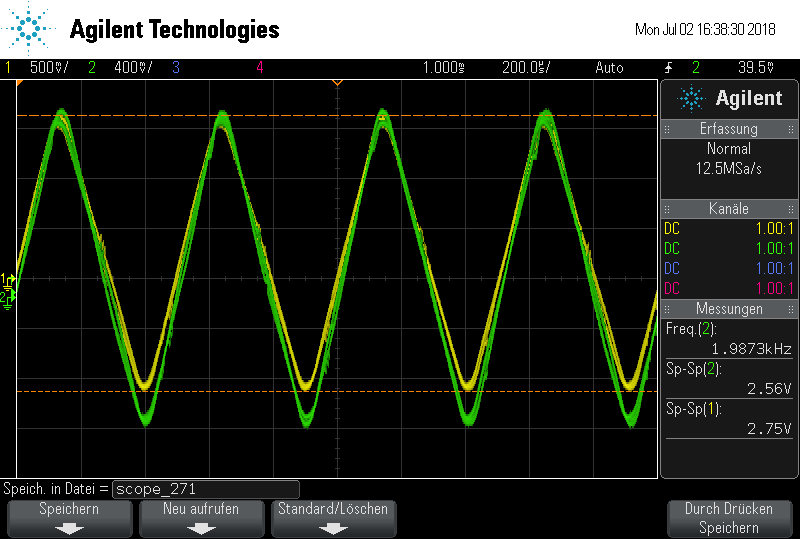
\includegraphics[height=0.3\textheight]{data/scope_271.png}
  \caption{Name}
  \label{fig:name}
\end{figure}

\subsection{Ged\"ampfte Schwingung}
\begin{figure}[ht]
  \centering
  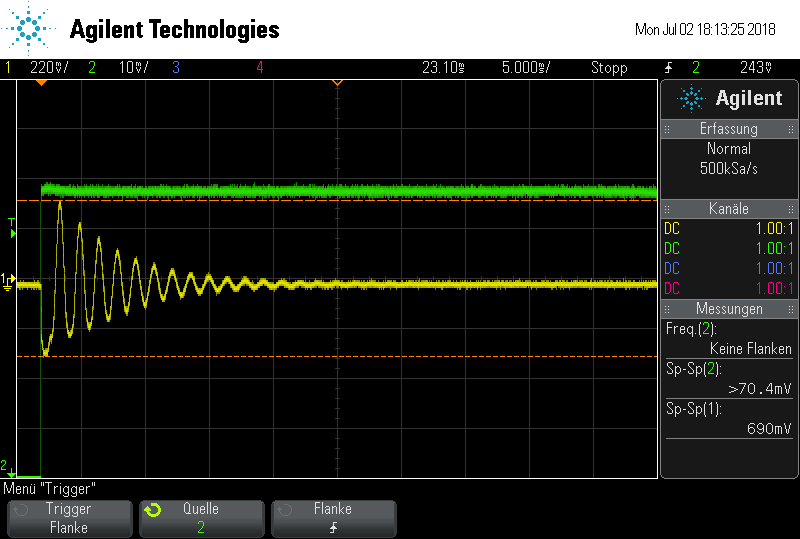
\includegraphics[height=0.3\textheight]{data/scope_275.png}
  \caption{Name}
  \label{fig:name}
\end{figure}
